\documentclass[10pt,twocolumn]{article}
\usepackage[a4paper,margin=0.85in]{geometry}
\setlength{\columnsep}{0.28in}
\raggedbottom

\usepackage[T1]{fontenc}
\usepackage[utf8]{inputenc}
\usepackage{lmodern}
\usepackage{amsmath,amssymb}
\usepackage{booktabs}
\usepackage{array}
\usepackage{graphicx}
\usepackage{tikz}
\usetikzlibrary{arrows.meta,positioning,fit,backgrounds,calc}
\usepackage{hyperref}
\hypersetup{
  colorlinks=true,
  linkcolor=black,
  citecolor=black,
  urlcolor=blue,
  pdftitle={ReproBot -- Third Progress Report},
  pdfauthor={Aleyna Kutuk, Engincan Varan, Gul Korkut, Goktug Mert Ozdogan}
}
\usepackage{xcolor}
\usepackage{caption}
\usepackage{pifont}

\definecolor{builtc}{HTML}{1B6F50}
\definecolor{missingc}{HTML}{97303F}
\definecolor{loopc}{HTML}{0E6E78}
\definecolor{warnc}{HTML}{97590C}

\newcommand{\built}{\textcolor{builtc}{\ding{51}}}
\newcommand{\absent}{\textcolor{missingc}{\ding{55}}}
\newcommand{\partl}{\textcolor{warnc}{$\sim$}}
\newcolumntype{L}[1]{>{\raggedright\arraybackslash}p{#1}}

\renewcommand{\topfraction}{0.9}
\renewcommand{\dbltopfraction}{0.9}
\renewcommand{\bottomfraction}{0.8}
\renewcommand{\textfraction}{0.07}
\renewcommand{\floatpagefraction}{0.75}
\renewcommand{\dblfloatpagefraction}{0.75}
\setcounter{topnumber}{3}
\setcounter{dbltopnumber}{3}
\setcounter{totalnumber}{5}

\title{\textbf{ReproBot: A Multi-Agent System for Automated Scientific Paper Replication}\\[0.4em]
\large Third Progress Report}
\author{
  Aleyna Kütük \\ \small\texttt{aleynakutuk10@gmail.com}
  \and
  Engincan Varan \\ \small\texttt{engincanvaran@gmail.com}
  \and
  Gül Korkut \\ \small\texttt{serifegulkorkut@gmail.com}
  \and
  Göktuğ Mert Özdoğan \\ \small\texttt{goekmeroz@gmail.com}
}
\date{inzva AI Projects \#10 \\ 13.09.2026}


\begin{document}

\maketitle

\begin{abstract}
ReproBot is a multi-agent system that reads a machine learning paper, extracts its claims and
experimental setup, generates an implementation, runs it in a sandbox, and repairs execution
failures through a bounded retry loop. This report presents its first full-fidelity
replications. We generalized code generation beyond image classification --- the Coder now
writes a plain PyTorch training loop for neural models and a scikit-learn estimator for
classical ones --- and evaluated on five papers whose original experiments train on a CPU,
spanning five model families: a network with a margin-based loss, a tabular regression network,
a kernel support vector machine, a random forest and a soft decision tree. For each we report
the learning curve of the generated implementation and a comparison with the published result.
Three reproductions agree closely with their papers: 0.82\% against 0.87\% MNIST test error, 96.63\% against 96.9\% SVM accuracy --- with the paper's own settings reproducing its numbers exactly --- and 87.73\% against 87.3\% random-forest accuracy; the soft decision tree was still training at the time of writing. A housing-price network reaches a test RMSE of 4.48 against 3.02, a gap we
trace to the paper's unspecified data split. The problems met along the way, from a misprinted
loss to a dead dataset link, were each resolved, three of them automatically by the retry loop.
We also present the team's first front end, a dashboard over the pipeline's outputs, and set out
the next phase: live checks on running training jobs, an automated Critic, and tighter control of
the retry loop.
\end{abstract}

\section{Introduction}
\label{sec:intro}

Reproducing a machine learning paper's reported results is mechanical in principle and
laborious in practice, and most published work ships no usable implementation. ReproBot
automates the process as a pipeline of specialized stages. A vision-language model converts
the paper's PDF into Markdown, reading figures as well as text. A Reader extracts five
structured fields --- a method summary, architecture notes, the claimed results, the
hyperparameters and the data pipeline --- and cross-checks them with a validation loop. A Coder
turns that extraction into a self-contained training script. A Runner executes the script in a
Docker container through four escalating stages: \texttt{probe}, a few optimizer steps;
\texttt{smoke}, one epoch on a small slice; \texttt{capped}, five epochs on a small slice; and
\texttt{full}, the paper's own setup. When a stage fails, a small model classifies the failure,
and an Orchestrator feeds that diagnosis back to the Coder and retries, within a fixed budget.

Before this phase the pipeline ran end to end but had only ever executed short checks: its
CIFAR-10 target papers need weeks of CPU time per full training run. This phase produced the
first full-fidelity results. Its contributions are:

\begin{itemize}
  \item a Coder that handles any supervised task and model family, writing PyTorch for neural
    networks and scikit-learn for classical estimators (Section~\ref{sec:pipeline});
  \item five complete replications across five model families, each with the implementation's
    learning curve and a comparison with the paper (Section~\ref{sec:results});
  \item a dashboard front end over the pipeline's outputs (Section~\ref{sec:viewer});
  \item a concrete plan for the next phase, grounded in what the runs showed
    (Section~\ref{sec:future}).
\end{itemize}

\section{Replication Targets}
\label{sec:targets}

Full training of the CIFAR-10 benchmark papers is out of reach on the project's hardware: one
\emph{Wide Residual Networks} run at the paper's setup measured at about 22 days on the
development CPU. Testing the pipeline's actual claim --- that a paper can be read, implemented,
executed and checked automatically --- needs only papers whose experiments are small. We chose
five that train in one minute to one hour, deliberately covering different model families and
data types (Table~\ref{tab:targets}), and kept them apart from the CIFAR-10 set.

\begin{table*}[tbp]
\centering
\small
\caption{The five replication targets of this phase.}
\label{tab:targets}
\begin{tabular}{L{0.26\textwidth}L{0.22\textwidth}L{0.2\textwidth}L{0.2\textwidth}}
\toprule
Paper & Model family & Data & Targeted claim \\
\midrule
Tang (2013) \cite{tang2013dlsvm} & MLP with an L2-SVM output layer & MNIST & 0.87\% test error \\
Wijaya (2023) \cite{wijaya2023housing} & Multi-branch dense network (Keras) & Boston Housing
  \cite{harrison1978hedonic}, tabular & Test RMSE 3.02 \\
Hsu, Chang and Lin (2003) \cite{hsu2003guide} & RBF support vector machine (LIBSVM
  \cite{chang2011libsvm}) & svmguide1, tabular & 96.9\% test accuracy \\
Xiao, Rasul and Vollgraf (2017) \cite{xiao2017fashion} & Random forest (scikit-learn
  \cite{pedregosa2011sklearn}) & Fashion-MNIST & 0.873 test accuracy, mean of 5 runs \\
Frosst and Hinton (2017) \cite{frosst2017soft} & Soft decision tree & MNIST & 94.45\% test
  accuracy \\
\bottomrule
\end{tabular}
\end{table*}

Two of the targets are classification networks, one a regression network, and two classical
methods. Tang's contribution is a loss function; Wijaya's model was written in Keras; the SVM
guide's result comes from a full model-selection procedure; the Fashion-MNIST figure is an
average over five runs; and the soft-tree paper states its tree depth but none of its training
settings. Each property exercises a different part of the pipeline.

\section{Pipeline Updates}
\label{sec:pipeline}


\begin{figure*}[tbp]
\centering
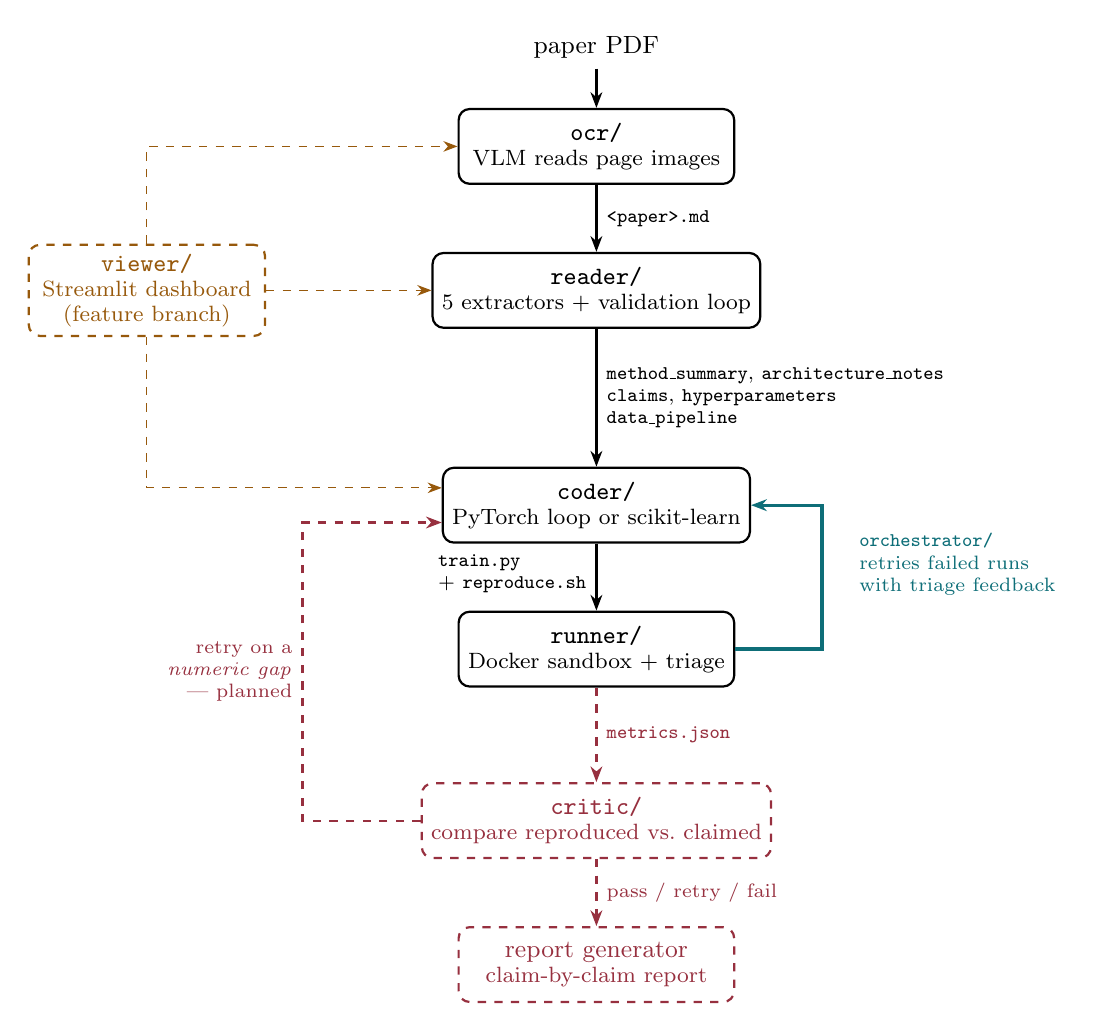
\begin{tikzpicture}[
  node distance=0.85cm and 1.5cm,
  stage/.style={draw, rounded corners, minimum width=3.5cm, minimum height=0.95cm,
    align=center, font=\small, thick},
  gone/.style={draw, rounded corners, minimum width=3.5cm, minimum height=0.95cm,
    align=center, font=\small, dashed, thick, draw=missingc, text=missingc},
  side/.style={draw, rounded corners, minimum width=3.0cm, minimum height=0.95cm,
    align=center, font=\small, thick, dashed, draw=warnc, text=warnc},
  arr/.style={-{Stealth[length=2mm]}, thick},
  gonearr/.style={-{Stealth[length=2mm]}, thick, dashed, draw=missingc},
  sidearr/.style={-{Stealth[length=1.8mm]}, dashed, draw=warnc},
  looparr/.style={-{Stealth[length=2mm]}, very thick, draw=loopc},
  lbl/.style={font=\scriptsize, align=left},
  gonelbl/.style={font=\scriptsize, align=left, text=missingc}
]
  \node[stage] (ocr)    {\texttt{ocr/}\\[-2pt]\footnotesize VLM reads page images};
  \node[stage, below=of ocr] (reader) {\texttt{reader/}\\[-2pt]\footnotesize 5 extractors + validation loop};
  \node[stage, below=1.75cm of reader] (coder) {\texttt{coder/}\\[-2pt]\footnotesize PyTorch loop or scikit-learn};
  \node[stage, below=of coder] (runner) {\texttt{runner/}\\[-2pt]\footnotesize Docker sandbox + triage};
  \node[gone,  below=1.2cm of runner] (critic) {\texttt{critic/}\\[-2pt]\footnotesize compare reproduced vs.\ claimed};
  \node[gone,  below=of critic] (report) {report generator\\[-2pt]\footnotesize claim-by-claim report};

  \node[above=0.5cm of ocr, font=\small, align=center] (pdf) {paper PDF};

  \node[side, left=2.1cm of reader] (viewer) {\texttt{viewer/}\\[-2pt]\footnotesize Streamlit dashboard\\[-2pt]\footnotesize (feature branch)};
  \draw[sidearr] (viewer.north) |- (ocr.west);
  \draw[sidearr] (viewer.east) -- (reader.west);
  \draw[sidearr] (viewer.south) |- ([yshift=0.22cm]coder.west);

  \draw[arr] (pdf) -- (ocr);
  \draw[arr] (ocr) -- node[right, lbl] {\texttt{<paper>.md}} (reader);
  \draw[arr] (reader) -- node[right, lbl]
    {\texttt{method\_summary}, \texttt{architecture\_notes}\\
     \texttt{claims}, \texttt{hyperparameters}\\ \texttt{data\_pipeline}} (coder);
  \draw[arr] (coder) -- node[left, lbl, pos=0.45] {\texttt{train.py}\\ + \texttt{reproduce.sh}} (runner);
  \draw[gonearr] (runner) -- node[right, gonelbl] {\texttt{metrics.json}} (critic);
  \draw[gonearr] (critic) -- node[right, gonelbl] {pass / retry / fail} (report);

  \draw[looparr] (runner.east) -- ++(1.1,0) |- (coder.east);
  \node[lbl, text=loopc, right=1.25cm of coder.east, anchor=west, yshift=-0.75cm]
    {\textbf{\texttt{orchestrator/}}\\ retries failed runs\\ with triage feedback};

  \draw[gonearr] (critic.west) -- ++(-1.5,0) |- node[pos=0.25, left, gonelbl, align=right]
    {retry on a\\ \emph{numeric gap}\\ --- planned} ([yshift=-0.22cm]coder.west);
\end{tikzpicture}
\caption{ReproBot on 13.09.2026. Solid components are built and verified by execution; dashed
red components are planned for the next phase; the dashed amber component is on a feature
branch. The Coder writes a PyTorch training loop or a scikit-learn estimator depending on the
paper's model family, and the Orchestrator retries failed runs by feeding the Runner's diagnosis
back to the Coder.}
\label{fig:pipeline}
\end{figure*}


\subsection{One training script for any model family}

\textbf{Neural models: a plain PyTorch loop.} The Coder previously emitted scripts built on
HuggingFace's \texttt{Trainer}, whose image-model interface suits neither a custom loss nor a
regression head. It now writes an explicit training loop in which the optimizer, schedule and
loss are all visible. When a paper was written in another framework, the Coder reproduces that
framework's defaults where the paper is silent --- Keras's Adam $\epsilon = 10^{-7}$, for
example --- and discloses each difference.

\textbf{Classical models: scikit-learn.} A support vector machine re-implemented as a PyTorch
model trained by gradient descent would use a different optimizer and reach a different
solution, so the Coder chooses its library by model family: SVMs, decision trees, forests,
$k$-nearest neighbours and linear models are scikit-learn estimators with every hyperparameter
passed by name, while networks --- including trees trained by gradient descent --- stay in
PyTorch. Because a paper's ``default parameters'' are those of the library version it used, the
Coder sets paper-era defaults explicitly; scikit-learn changed several in version 0.22.

\textbf{A common contract.} Every script accepts the same command-line flags, so the Runner
needs no per-paper logic, and writes the same metrics file: the claim's own metric on the
training and test splits, the metric's direction, the task type, and, when the claim is an
average over runs or folds, every run's value. Data comes from stable sources ---
\texttt{torchvision}, OpenML or the paper's own dataset site --- and each script checks the
dataset's name and shape before training on it.

\subsection{Problems encountered and how we solved them}

Table~\ref{tab:problems} lists the problems the replications surfaced and the fix applied to
each. Three were runtime defects in generated code that the retry loop repaired without human
involvement; the rest led to permanent changes in the prompts or the pipeline, or to a
documented correction.

\begin{table*}[tbp]
\centering
\small
\caption{Problems encountered during the replications, and how each was solved.}
\label{tab:problems}
\begin{tabular}{L{0.44\textwidth}L{0.48\textwidth}}
\toprule
Problem & Solution \\
\midrule
HuggingFace \texttt{Trainer} silently applied gradient clipping that no paper states
  & Explicit PyTorch training loop; every setting written down \\
Re-implementing classical models in PyTorch would change their solver
  & Library chosen by model family; scikit-learn with paper-era defaults \\
A remembered dataset URL had gone dead (HTTP 403), and triage filed it as an environment fault
  & OpenML first; triage treats one refusing source as a fixable script error \\
Dataset identifiers recalled from memory can name the wrong dataset
  & No identifiers from memory; scripts assert the dataset's name and shape \\
Tang: two unstated defaults (momentum 0.9, $C = 1.0$) together destabilized training at full
  scale & A six-configuration ablation isolated the pair; $C = 0.1$ trains stably \\
Soft tree: the paper prints its loss as the logarithm of a non-positive quantity
  & Implemented the evident intent, the expected cross-entropy \\
Runtime defects: a wrong API call (Wijaya), a label-sorted data file (SVM), an in-place
  autograd operation (soft tree) & Repaired automatically by the retry loop, one retry each \\
A dataset paper has no ``own method'', so the first claims extraction was empty (Fashion-MNIST)
  & The validation loop flagged it; the retry extracted 26 claims \\
The full stage wrote its metrics under a different filename than the Runner reads
  & Script template corrected \\
\bottomrule
\end{tabular}
\end{table*}

\subsection{The retry loop in action}


\begin{figure*}[tbp]
\centering
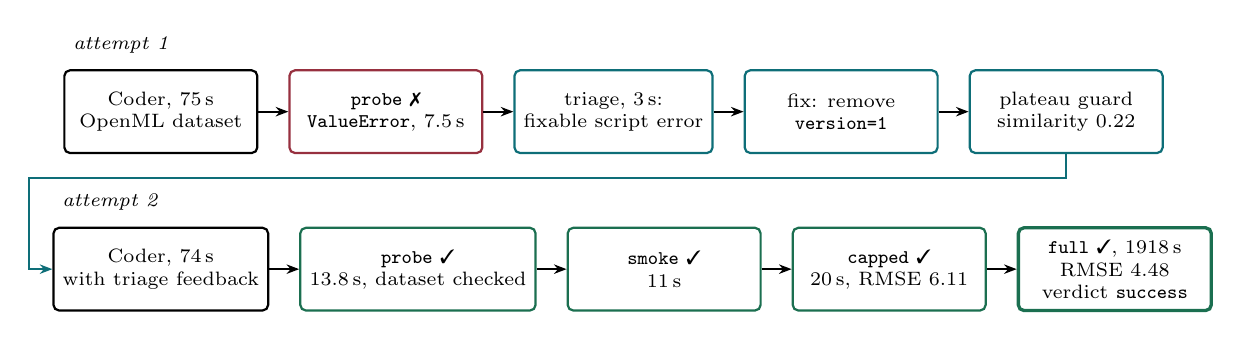
\begin{tikzpicture}[
  st/.style={draw, rounded corners=2pt, minimum width=2.45cm, minimum height=1.05cm,
    align=center, font=\scriptsize, thick},
  ok/.style={st, draw=builtc},
  bad/.style={st, draw=missingc},
  tri/.style={st, draw=loopc},
  arr/.style={-{Stealth[length=1.6mm]}, thick},
  row/.style={font=\scriptsize\itshape, anchor=south west}
]
  \node[st] (a1) at (0,0) {Coder, 75\,s\\ OpenML dataset};
  \node[bad, right=0.38cm of a1] (b1) {\texttt{probe} \ding{55}\\ \texttt{ValueError}, 7.5\,s};
  \node[tri, right=0.38cm of b1] (c1) {triage, 3\,s:\\ fixable script error};
  \node[tri, right=0.38cm of c1] (d1) {fix: remove\\ \texttt{version=1}};
  \node[tri, right=0.38cm of d1] (e1) {plateau guard\\ similarity 0.22};
  \draw[arr] (a1) -- (b1); \draw[arr] (b1) -- (c1); \draw[arr] (c1) -- (d1); \draw[arr] (d1) -- (e1);
  \node[row] at ([yshift=0.08cm]a1.north west) {attempt 1};

  \node[st] (a2) at (0,-2.0) {Coder, 74\,s\\ with triage feedback};
  \node[ok, right=0.38cm of a2] (b2) {\texttt{probe} \ding{51}\\ 13.8\,s, dataset checked};
  \node[ok, right=0.38cm of b2] (c2) {\texttt{smoke} \ding{51}\\ 11\,s};
  \node[ok, right=0.38cm of c2] (d2) {\texttt{capped} \ding{51}\\ 20\,s, RMSE 6.11};
  \node[ok, right=0.38cm of d2, line width=1.2pt] (e2) {\texttt{full} \ding{51}, 1918\,s\\ RMSE 4.48\\ verdict \texttt{success}};
  \draw[arr] (a2) -- (b2); \draw[arr] (b2) -- (c2); \draw[arr] (c2) -- (d2); \draw[arr] (d2) -- (e2);
  \node[row] at ([yshift=0.08cm]a2.north west) {attempt 2};

  \draw[arr, draw=loopc] (e1.south) -- ++(0,-0.3) -| ([xshift=-0.3cm]a2.west) -- (a2.west);
\end{tikzpicture}
\caption{An automatic repair by the retry loop, on the housing-price paper. The first script
failed its first check; triage diagnosed a fixable script error, the Coder regenerated the script
with that feedback, and the second attempt passed every stage through the full run.}
\label{fig:wijayarun}
\end{figure*}


Figure~\ref{fig:wijayarun} shows a typical automatic repair. The first generated script for
the housing-price paper passed two conflicting arguments to scikit-learn's dataset loader and
stopped within seconds. Triage classified the failure as a fixable script error and proposed
removing one argument; the Coder regenerated the script with that feedback, and the second
attempt passed every stage through the full run. The SVM and soft-tree scripts were repaired
the same way. A plateau guard, which compares each regenerated script with its predecessor to
stop a loop that is not changing anything, measured similarities of 0.22 to 0.27, far from its
0.98 stopping threshold.

\section{Results}
\label{sec:results}

\subsection{Overview}

Table~\ref{tab:results} compares each reproduction with its paper, and
Figure~\ref{fig:curves} shows the learning curve of each generated implementation. All five
scripts were generated by the Coder and executed by the Runner at the papers' full settings.
Two needed a manual correction before their final run, listed in Table~\ref{tab:problems}: one
unstated hyperparameter for Tang, and the misprinted loss for the soft tree.

\begin{table*}[tbp]
\centering
\small
\caption{Reproduced results against the published claims. Runtimes are the full stage's wall
clock on the development CPU.}
\label{tab:results}
\begin{tabular}{L{0.19\textwidth}L{0.2\textwidth}rrrL{0.2\textwidth}}
\toprule
Paper & Claim & Paper & ReproBot & Runtime & Agreement \\
\midrule
Tang (2013) & MNIST test error & 0.87\% & \textbf{0.82\%} & 54\,min & Within 0.05 points \\
Wijaya (2023) & Boston Housing test RMSE & 3.02 & \textbf{4.48} & 32\,min & Not matched; train
  RMSE 2.94 vs 2.69 \\
Hsu et al.\ (2003) & svmguide1 test accuracy & 96.9\% & \textbf{96.63\%} & 73\,s & Within 0.3
  points; exact at the paper's settings \\
Xiao et al.\ (2017) & Fashion-MNIST accuracy, mean of 5 runs & 0.873 & \textbf{0.8773} &
  3.3\,min & Within 0.5 points \\
Frosst and Hinton (2017) & MNIST test accuracy & 94.45\% & \textbf{(running)} &
  --- & Pending \\
\bottomrule
\end{tabular}
\end{table*}


\begin{figure*}[tbp]
\centering
\begin{minipage}[t]{0.49\linewidth}\centering
\resizebox{0.97\linewidth}{!}{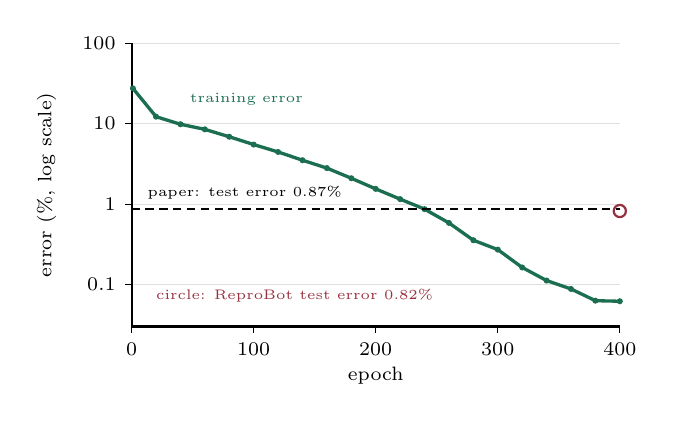
\begin{tikzpicture}
  \draw[black!12] (0,0.534) -- (6.2,0.534);
  \draw (0,0.534) -- (-0.08,0.534) node[left, font=\scriptsize] {0.1};
  \draw[black!12] (0,1.556) -- (6.2,1.556);
  \draw (0,1.556) -- (-0.08,1.556) node[left, font=\scriptsize] {1};
  \draw[black!12] (0,2.578) -- (6.2,2.578);
  \draw (0,2.578) -- (-0.08,2.578) node[left, font=\scriptsize] {10};
  \draw[black!12] (0,3.600) -- (6.2,3.600);
  \draw (0,3.600) -- (-0.08,3.600) node[left, font=\scriptsize] {100};
  \draw (0.000,0) -- (0.000,-0.08) node[below, font=\scriptsize] {0};
  \draw (1.550,0) -- (1.550,-0.08) node[below, font=\scriptsize] {100};
  \draw (3.100,0) -- (3.100,-0.08) node[below, font=\scriptsize] {200};
  \draw (4.650,0) -- (4.650,-0.08) node[below, font=\scriptsize] {300};
  \draw (6.200,0) -- (6.200,-0.08) node[below, font=\scriptsize] {400};
  \draw[thick] (0,0) -- (6.2,0);
  \draw[thick] (0,0) -- (0,3.6);
  \node[font=\scriptsize] at (3.100,-0.62) {epoch};
  \node[font=\scriptsize, rotate=90] at (-1.08,1.800) {error (\%, log scale)};
  \draw[builtc, very thick] (0.016,3.026) -- (0.310,2.666) -- (0.620,2.570) -- (0.930,2.505) -- (1.240,2.411) -- (1.550,2.312) -- (1.860,2.218) -- (2.170,2.113) -- (2.480,2.013) -- (2.790,1.884) -- (3.100,1.749) -- (3.410,1.619) -- (3.720,1.492) -- (4.030,1.317) -- (4.340,1.097) -- (4.650,0.978) -- (4.960,0.751) -- (5.270,0.585) -- (5.580,0.478) -- (5.890,0.329) -- (6.200,0.322);
  \fill[builtc] (0.016,3.026) circle (1.1pt);
  \fill[builtc] (0.310,2.666) circle (1.1pt);
  \fill[builtc] (0.620,2.570) circle (1.1pt);
  \fill[builtc] (0.930,2.505) circle (1.1pt);
  \fill[builtc] (1.240,2.411) circle (1.1pt);
  \fill[builtc] (1.550,2.312) circle (1.1pt);
  \fill[builtc] (1.860,2.218) circle (1.1pt);
  \fill[builtc] (2.170,2.113) circle (1.1pt);
  \fill[builtc] (2.480,2.013) circle (1.1pt);
  \fill[builtc] (2.790,1.884) circle (1.1pt);
  \fill[builtc] (3.100,1.749) circle (1.1pt);
  \fill[builtc] (3.410,1.619) circle (1.1pt);
  \fill[builtc] (3.720,1.492) circle (1.1pt);
  \fill[builtc] (4.030,1.317) circle (1.1pt);
  \fill[builtc] (4.340,1.097) circle (1.1pt);
  \fill[builtc] (4.650,0.978) circle (1.1pt);
  \fill[builtc] (4.960,0.751) circle (1.1pt);
  \fill[builtc] (5.270,0.585) circle (1.1pt);
  \fill[builtc] (5.580,0.478) circle (1.1pt);
  \fill[builtc] (5.890,0.329) circle (1.1pt);
  \fill[builtc] (6.200,0.322) circle (1.1pt);
  \draw[black, densely dashed] (0,1.494) -- (6.2,1.494);
  \node[font=\tiny, anchor=south west, text=black] at (0.080,1.494) {paper: test error 0.87\%};
  \draw[missingc, thick] (6.200,1.468) circle (2.2pt);
  \node[font=\tiny, text=missingc, anchor=south west] at (0.186,0.180)
    {circle: ReproBot test error 0.82\%};
  \node[font=\tiny, text=builtc, anchor=west] at (0.620,2.886) {training error};
\end{tikzpicture}}\\[-1pt]
{\small (a) MLP with L2-SVM loss, MNIST}
\end{minipage}
\hfill
\begin{minipage}[t]{0.49\linewidth}\centering
\resizebox{0.97\linewidth}{!}{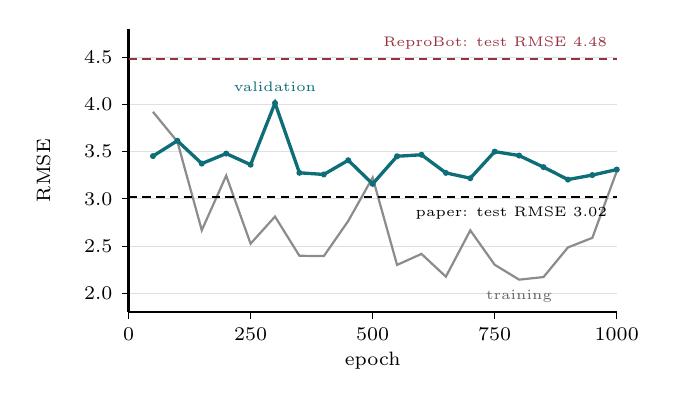
\begin{tikzpicture}
  \draw[black!12] (0,0.240) -- (6.2,0.240);
  \draw (0,0.240) -- (-0.08,0.240) node[left, font=\scriptsize] {2.0};
  \draw[black!12] (0,0.840) -- (6.2,0.840);
  \draw (0,0.840) -- (-0.08,0.840) node[left, font=\scriptsize] {2.5};
  \draw[black!12] (0,1.440) -- (6.2,1.440);
  \draw (0,1.440) -- (-0.08,1.440) node[left, font=\scriptsize] {3.0};
  \draw[black!12] (0,2.040) -- (6.2,2.040);
  \draw (0,2.040) -- (-0.08,2.040) node[left, font=\scriptsize] {3.5};
  \draw[black!12] (0,2.640) -- (6.2,2.640);
  \draw (0,2.640) -- (-0.08,2.640) node[left, font=\scriptsize] {4.0};
  \draw[black!12] (0,3.240) -- (6.2,3.240);
  \draw (0,3.240) -- (-0.08,3.240) node[left, font=\scriptsize] {4.5};
  \draw (0.000,0) -- (0.000,-0.08) node[below, font=\scriptsize] {0};
  \draw (1.550,0) -- (1.550,-0.08) node[below, font=\scriptsize] {250};
  \draw (3.100,0) -- (3.100,-0.08) node[below, font=\scriptsize] {500};
  \draw (4.650,0) -- (4.650,-0.08) node[below, font=\scriptsize] {750};
  \draw (6.200,0) -- (6.200,-0.08) node[below, font=\scriptsize] {1000};
  \draw[thick] (0,0) -- (6.2,0);
  \draw[thick] (0,0) -- (0,3.6);
  \node[font=\scriptsize] at (3.100,-0.62) {epoch};
  \node[font=\scriptsize, rotate=90] at (-1.08,1.800) {RMSE};
  \draw[black!45, thick] (0.310,2.545) -- (0.620,2.167) -- (0.930,1.041) -- (1.240,1.735) -- (1.550,0.871) -- (1.860,1.215) -- (2.170,0.717) -- (2.480,0.713) -- (2.790,1.159) -- (3.100,1.711) -- (3.410,0.601) -- (3.720,0.741) -- (4.030,0.452) -- (4.340,1.040) -- (4.650,0.603) -- (4.960,0.414) -- (5.270,0.447) -- (5.580,0.823) -- (5.890,0.945) -- (6.200,1.790);
  \draw[loopc, very thick] (0.310,1.983) -- (0.620,2.178) -- (0.930,1.888) -- (1.240,2.015) -- (1.550,1.874) -- (1.860,2.657) -- (2.170,1.771) -- (2.480,1.750) -- (2.790,1.930) -- (3.100,1.630) -- (3.410,1.981) -- (3.720,2.000) -- (4.030,1.770) -- (4.340,1.702) -- (4.650,2.040) -- (4.960,1.990) -- (5.270,1.843) -- (5.580,1.685) -- (5.890,1.742) -- (6.200,1.812);
  \fill[loopc] (0.310,1.983) circle (1.1pt);
  \fill[loopc] (0.620,2.178) circle (1.1pt);
  \fill[loopc] (0.930,1.888) circle (1.1pt);
  \fill[loopc] (1.240,2.015) circle (1.1pt);
  \fill[loopc] (1.550,1.874) circle (1.1pt);
  \fill[loopc] (1.860,2.657) circle (1.1pt);
  \fill[loopc] (2.170,1.771) circle (1.1pt);
  \fill[loopc] (2.480,1.750) circle (1.1pt);
  \fill[loopc] (2.790,1.930) circle (1.1pt);
  \fill[loopc] (3.100,1.630) circle (1.1pt);
  \fill[loopc] (3.410,1.981) circle (1.1pt);
  \fill[loopc] (3.720,2.000) circle (1.1pt);
  \fill[loopc] (4.030,1.770) circle (1.1pt);
  \fill[loopc] (4.340,1.702) circle (1.1pt);
  \fill[loopc] (4.650,2.040) circle (1.1pt);
  \fill[loopc] (4.960,1.990) circle (1.1pt);
  \fill[loopc] (5.270,1.843) circle (1.1pt);
  \fill[loopc] (5.580,1.685) circle (1.1pt);
  \fill[loopc] (5.890,1.742) circle (1.1pt);
  \fill[loopc] (6.200,1.812) circle (1.1pt);
  \draw[black, densely dashed] (0,1.464) -- (6.2,1.464);
  \node[font=\tiny, anchor=north east, text=black] at (6.200,1.464) {paper: test RMSE 3.02};
  \draw[missingc, densely dashed] (0,3.216) -- (6.2,3.216);
  \node[font=\tiny, anchor=south east, text=missingc] at (6.200,3.216) {ReproBot: test RMSE 4.48};
  \node[font=\tiny, text=loopc, anchor=south] at (1.860,2.682)
    {validation};
  \node[font=\tiny, text=black!60, anchor=north] at (4.960,0.400)
    {training};
\end{tikzpicture}}\\[-1pt]
{\small (b) Dense network, Boston Housing}
\end{minipage}
\\[10pt]
\begin{minipage}[t]{0.49\linewidth}\centering
\resizebox{0.97\linewidth}{!}{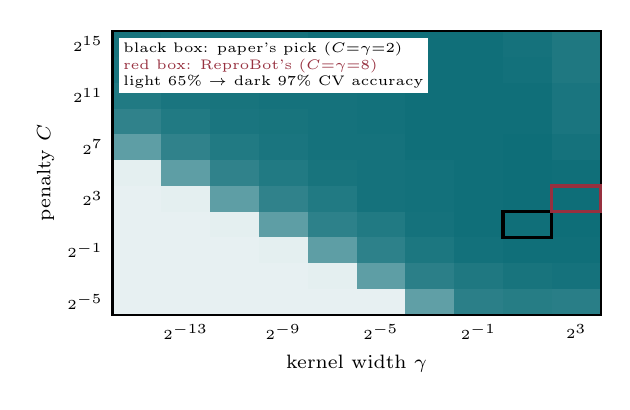
\begin{tikzpicture}
  \fill[loopc!10!white] (0.000,0.000) rectangle (0.620,0.327);
  \fill[loopc!10!white] (0.620,0.000) rectangle (1.240,0.327);
  \fill[loopc!10!white] (1.240,0.000) rectangle (1.860,0.327);
  \fill[loopc!10!white] (1.860,0.000) rectangle (2.480,0.327);
  \fill[loopc!10!white] (2.480,0.000) rectangle (3.100,0.327);
  \fill[loopc!10!white] (3.100,0.000) rectangle (3.720,0.327);
  \fill[loopc!66!white] (3.720,0.000) rectangle (4.340,0.327);
  \fill[loopc!88!white] (4.340,0.000) rectangle (4.960,0.327);
  \fill[loopc!90!white] (4.960,0.000) rectangle (5.580,0.327);
  \fill[loopc!89!white] (5.580,0.000) rectangle (6.200,0.327);
  \fill[loopc!10!white] (0.000,0.327) rectangle (0.620,0.655);
  \fill[loopc!10!white] (0.620,0.327) rectangle (1.240,0.655);
  \fill[loopc!10!white] (1.240,0.327) rectangle (1.860,0.655);
  \fill[loopc!10!white] (1.860,0.327) rectangle (2.480,0.655);
  \fill[loopc!11!white] (2.480,0.327) rectangle (3.100,0.655);
  \fill[loopc!67!white] (3.100,0.327) rectangle (3.720,0.655);
  \fill[loopc!88!white] (3.720,0.327) rectangle (4.340,0.655);
  \fill[loopc!93!white] (4.340,0.327) rectangle (4.960,0.655);
  \fill[loopc!96!white] (4.960,0.327) rectangle (5.580,0.655);
  \fill[loopc!97!white] (5.580,0.327) rectangle (6.200,0.655);
  \fill[loopc!10!white] (0.000,0.655) rectangle (0.620,0.982);
  \fill[loopc!10!white] (0.620,0.655) rectangle (1.240,0.982);
  \fill[loopc!10!white] (1.240,0.655) rectangle (1.860,0.982);
  \fill[loopc!11!white] (1.860,0.655) rectangle (2.480,0.982);
  \fill[loopc!67!white] (2.480,0.655) rectangle (3.100,0.982);
  \fill[loopc!87!white] (3.100,0.655) rectangle (3.720,0.982);
  \fill[loopc!94!white] (3.720,0.655) rectangle (4.340,0.982);
  \fill[loopc!98!white] (4.340,0.655) rectangle (4.960,0.982);
  \fill[loopc!99!white] (4.960,0.655) rectangle (5.580,0.982);
  \fill[loopc!99!white] (5.580,0.655) rectangle (6.200,0.982);
  \fill[loopc!10!white] (0.000,0.982) rectangle (0.620,1.309);
  \fill[loopc!10!white] (0.620,0.982) rectangle (1.240,1.309);
  \fill[loopc!11!white] (1.240,0.982) rectangle (1.860,1.309);
  \fill[loopc!67!white] (1.860,0.982) rectangle (2.480,1.309);
  \fill[loopc!87!white] (2.480,0.982) rectangle (3.100,1.309);
  \fill[loopc!92!white] (3.100,0.982) rectangle (3.720,1.309);
  \fill[loopc!97!white] (3.720,0.982) rectangle (4.340,1.309);
  \fill[loopc!99!white] (4.340,0.982) rectangle (4.960,1.309);
  \fill[loopc!99!white] (4.960,0.982) rectangle (5.580,1.309);
  \fill[loopc!100!white] (5.580,0.982) rectangle (6.200,1.309);
  \fill[loopc!10!white] (0.000,1.309) rectangle (0.620,1.636);
  \fill[loopc!11!white] (0.620,1.309) rectangle (1.240,1.636);
  \fill[loopc!67!white] (1.240,1.309) rectangle (1.860,1.636);
  \fill[loopc!86!white] (1.860,1.309) rectangle (2.480,1.636);
  \fill[loopc!92!white] (2.480,1.309) rectangle (3.100,1.636);
  \fill[loopc!97!white] (3.100,1.309) rectangle (3.720,1.636);
  \fill[loopc!98!white] (3.720,1.309) rectangle (4.340,1.636);
  \fill[loopc!99!white] (4.340,1.309) rectangle (4.960,1.636);
  \fill[loopc!100!white] (4.960,1.309) rectangle (5.580,1.636);
  \fill[loopc!100!white] (5.580,1.309) rectangle (6.200,1.636);
  \fill[loopc!11!white] (0.000,1.636) rectangle (0.620,1.964);
  \fill[loopc!67!white] (0.620,1.636) rectangle (1.240,1.964);
  \fill[loopc!86!white] (1.240,1.636) rectangle (1.860,1.964);
  \fill[loopc!92!white] (1.860,1.636) rectangle (2.480,1.964);
  \fill[loopc!96!white] (2.480,1.636) rectangle (3.100,1.964);
  \fill[loopc!97!white] (3.100,1.636) rectangle (3.720,1.964);
  \fill[loopc!98!white] (3.720,1.636) rectangle (4.340,1.964);
  \fill[loopc!99!white] (4.340,1.636) rectangle (4.960,1.964);
  \fill[loopc!100!white] (4.960,1.636) rectangle (5.580,1.964);
  \fill[loopc!99!white] (5.580,1.636) rectangle (6.200,1.964);
  \fill[loopc!67!white] (0.000,1.964) rectangle (0.620,2.291);
  \fill[loopc!86!white] (0.620,1.964) rectangle (1.240,2.291);
  \fill[loopc!92!white] (1.240,1.964) rectangle (1.860,2.291);
  \fill[loopc!95!white] (1.860,1.964) rectangle (2.480,2.291);
  \fill[loopc!97!white] (2.480,1.964) rectangle (3.100,2.291);
  \fill[loopc!97!white] (3.100,1.964) rectangle (3.720,2.291);
  \fill[loopc!99!white] (3.720,1.964) rectangle (4.340,2.291);
  \fill[loopc!99!white] (4.340,1.964) rectangle (4.960,2.291);
  \fill[loopc!100!white] (4.960,1.964) rectangle (5.580,2.291);
  \fill[loopc!97!white] (5.580,1.964) rectangle (6.200,2.291);
  \fill[loopc!86!white] (0.000,2.291) rectangle (0.620,2.618);
  \fill[loopc!92!white] (0.620,2.291) rectangle (1.240,2.618);
  \fill[loopc!95!white] (1.240,2.291) rectangle (1.860,2.618);
  \fill[loopc!96!white] (1.860,2.291) rectangle (2.480,2.618);
  \fill[loopc!97!white] (2.480,2.291) rectangle (3.100,2.618);
  \fill[loopc!98!white] (3.100,2.291) rectangle (3.720,2.618);
  \fill[loopc!99!white] (3.720,2.291) rectangle (4.340,2.618);
  \fill[loopc!99!white] (4.340,2.291) rectangle (4.960,2.618);
  \fill[loopc!99!white] (4.960,2.291) rectangle (5.580,2.618);
  \fill[loopc!95!white] (5.580,2.291) rectangle (6.200,2.618);
  \fill[loopc!92!white] (0.000,2.618) rectangle (0.620,2.945);
  \fill[loopc!95!white] (0.620,2.618) rectangle (1.240,2.945);
  \fill[loopc!96!white] (1.240,2.618) rectangle (1.860,2.945);
  \fill[loopc!97!white] (1.860,2.618) rectangle (2.480,2.945);
  \fill[loopc!97!white] (2.480,2.618) rectangle (3.100,2.945);
  \fill[loopc!98!white] (3.100,2.618) rectangle (3.720,2.945);
  \fill[loopc!99!white] (3.720,2.618) rectangle (4.340,2.945);
  \fill[loopc!99!white] (4.340,2.618) rectangle (4.960,2.945);
  \fill[loopc!99!white] (4.960,2.618) rectangle (5.580,2.945);
  \fill[loopc!95!white] (5.580,2.618) rectangle (6.200,2.945);
  \fill[loopc!95!white] (0.000,2.945) rectangle (0.620,3.273);
  \fill[loopc!95!white] (0.620,2.945) rectangle (1.240,3.273);
  \fill[loopc!95!white] (1.240,2.945) rectangle (1.860,3.273);
  \fill[loopc!97!white] (1.860,2.945) rectangle (2.480,3.273);
  \fill[loopc!98!white] (2.480,2.945) rectangle (3.100,3.273);
  \fill[loopc!99!white] (3.100,2.945) rectangle (3.720,3.273);
  \fill[loopc!99!white] (3.720,2.945) rectangle (4.340,3.273);
  \fill[loopc!99!white] (4.340,2.945) rectangle (4.960,3.273);
  \fill[loopc!98!white] (4.960,2.945) rectangle (5.580,3.273);
  \fill[loopc!93!white] (5.580,2.945) rectangle (6.200,3.273);
  \fill[loopc!96!white] (0.000,3.273) rectangle (0.620,3.600);
  \fill[loopc!95!white] (0.620,3.273) rectangle (1.240,3.600);
  \fill[loopc!97!white] (1.240,3.273) rectangle (1.860,3.600);
  \fill[loopc!97!white] (1.860,3.273) rectangle (2.480,3.600);
  \fill[loopc!99!white] (2.480,3.273) rectangle (3.100,3.600);
  \fill[loopc!99!white] (3.100,3.273) rectangle (3.720,3.600);
  \fill[loopc!99!white] (3.720,3.273) rectangle (4.340,3.600);
  \fill[loopc!99!white] (4.340,3.273) rectangle (4.960,3.600);
  \fill[loopc!97!white] (4.960,3.273) rectangle (5.580,3.600);
  \fill[loopc!93!white] (5.580,3.273) rectangle (6.200,3.600);
  \draw[thick] (0,0) rectangle (6.2,3.6);
  \node[font=\tiny, below] at (0.930,0) {$2^{-13}$};
  \node[font=\tiny, below] at (2.170,0) {$2^{-9}$};
  \node[font=\tiny, below] at (3.410,0) {$2^{-5}$};
  \node[font=\tiny, below] at (4.650,0) {$2^{-1}$};
  \node[font=\tiny, below] at (5.890,0) {$2^{3}$};
  \node[font=\tiny, left] at (0,0.164) {$2^{-5}$};
  \node[font=\tiny, left] at (0,0.818) {$2^{-1}$};
  \node[font=\tiny, left] at (0,1.473) {$2^{3}$};
  \node[font=\tiny, left] at (0,2.127) {$2^{7}$};
  \node[font=\tiny, left] at (0,2.782) {$2^{11}$};
  \node[font=\tiny, left] at (0,3.436) {$2^{15}$};
  \draw[black, very thick] (4.960,0.982)
    rectangle (5.580,1.309);
  \draw[missingc, very thick] (5.580,1.309)
    rectangle (6.200,1.636);
  \node[font=\scriptsize] at (3.100,-0.62) {kernel width $\gamma$};
  \node[font=\scriptsize, rotate=90] at (-0.85,1.800) {penalty $C$};
  \node[font=\tiny, anchor=north west, fill=white, inner sep=1.5pt, align=left]
    at (0.08,3.520)
    {black box: paper's pick ($C{=}\gamma{=}2$)\\
      \textcolor{missingc}{red box: ReproBot's ($C{=}\gamma{=}8$)}\\
      light 65\% $\to$ dark 97\% CV accuracy};
\end{tikzpicture}}\\[-1pt]
{\small (c) RBF SVM model selection, svmguide1}
\end{minipage}
\hfill
\begin{minipage}[t]{0.49\linewidth}\centering
\resizebox{0.97\linewidth}{!}{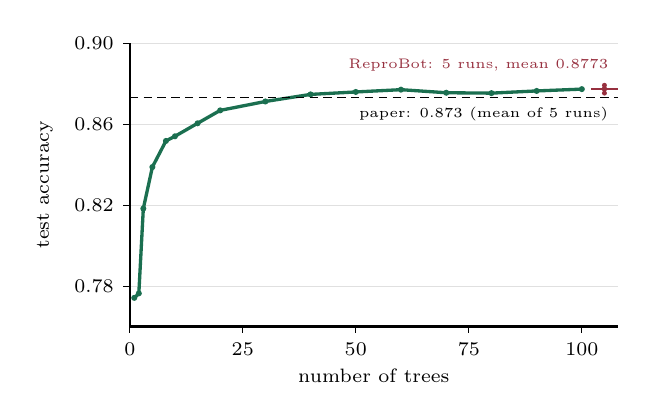
\begin{tikzpicture}
  \draw[black!12] (0,0.514) -- (6.2,0.514);
  \draw (0,0.514) -- (-0.08,0.514) node[left, font=\scriptsize] {0.78};
  \draw[black!12] (0,1.543) -- (6.2,1.543);
  \draw (0,1.543) -- (-0.08,1.543) node[left, font=\scriptsize] {0.82};
  \draw[black!12] (0,2.571) -- (6.2,2.571);
  \draw (0,2.571) -- (-0.08,2.571) node[left, font=\scriptsize] {0.86};
  \draw[black!12] (0,3.600) -- (6.2,3.600);
  \draw (0,3.600) -- (-0.08,3.600) node[left, font=\scriptsize] {0.90};
  \draw (0.000,0) -- (0.000,-0.08) node[below, font=\scriptsize] {0};
  \draw (1.435,0) -- (1.435,-0.08) node[below, font=\scriptsize] {25};
  \draw (2.870,0) -- (2.870,-0.08) node[below, font=\scriptsize] {50};
  \draw (4.306,0) -- (4.306,-0.08) node[below, font=\scriptsize] {75};
  \draw (5.741,0) -- (5.741,-0.08) node[below, font=\scriptsize] {100};
  \draw[thick] (0,0) -- (6.2,0);
  \draw[thick] (0,0) -- (0,3.6);
  \node[font=\scriptsize] at (3.100,-0.62) {number of trees};
  \node[font=\scriptsize, rotate=90] at (-1.08,1.800) {test accuracy};
  \draw[builtc, very thick] (0.057,0.365) -- (0.115,0.422) -- (0.172,1.499) -- (0.287,2.026) -- (0.459,2.358) -- (0.574,2.417) -- (0.861,2.582) -- (1.148,2.746) -- (1.722,2.859) -- (2.296,2.949) -- (2.870,2.980) -- (3.444,3.009) -- (4.019,2.970) -- (4.593,2.965) -- (5.167,2.993) -- (5.741,3.016);
  \fill[builtc] (0.057,0.365) circle (1.1pt);
  \fill[builtc] (0.115,0.422) circle (1.1pt);
  \fill[builtc] (0.172,1.499) circle (1.1pt);
  \fill[builtc] (0.287,2.026) circle (1.1pt);
  \fill[builtc] (0.459,2.358) circle (1.1pt);
  \fill[builtc] (0.574,2.417) circle (1.1pt);
  \fill[builtc] (0.861,2.582) circle (1.1pt);
  \fill[builtc] (1.148,2.746) circle (1.1pt);
  \fill[builtc] (1.722,2.859) circle (1.1pt);
  \fill[builtc] (2.296,2.949) circle (1.1pt);
  \fill[builtc] (2.870,2.980) circle (1.1pt);
  \fill[builtc] (3.444,3.009) circle (1.1pt);
  \fill[builtc] (4.019,2.970) circle (1.1pt);
  \fill[builtc] (4.593,2.965) circle (1.1pt);
  \fill[builtc] (5.167,2.993) circle (1.1pt);
  \fill[builtc] (5.741,3.016) circle (1.1pt);
  \draw[black, densely dashed] (0,2.906) -- (6.2,2.906);
  \node[font=\tiny, anchor=north east, text=black] at (6.200,2.906) {paper: 0.873 (mean of 5 runs)};
  \fill[missingc] (6.028,3.016) circle (0.9pt);
  \fill[missingc] (6.028,3.019) circle (0.9pt);
  \fill[missingc] (6.028,2.965) circle (0.9pt);
  \fill[missingc] (6.028,3.065) circle (0.9pt);
  \fill[missingc] (6.028,3.021) circle (0.9pt);
  \draw[missingc, thick] (5.856,3.017) -- (6.200,3.017);
  \node[font=\tiny, text=missingc, anchor=south east] at (6.200,3.115)
    {ReproBot: 5 runs, mean 0.8773};
\end{tikzpicture}}\\[-1pt]
{\small (d) Random forest, Fashion-MNIST}
\end{minipage}
\\[10pt]
\begin{minipage}[t]{0.49\linewidth}\centering
\resizebox{0.97\linewidth}{!}{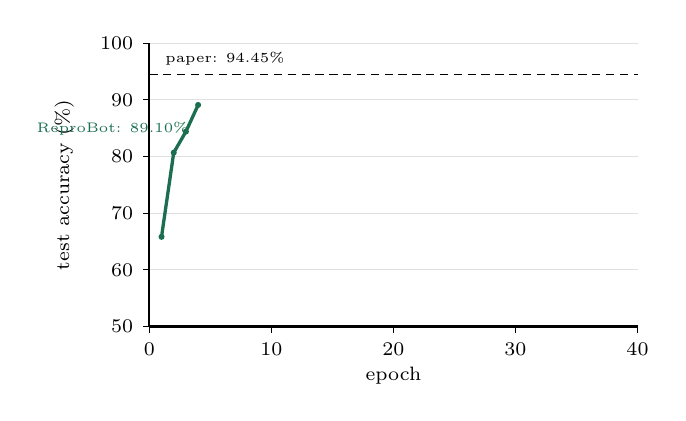
\begin{tikzpicture}
  \draw[black!12] (0,0.000) -- (6.2,0.000);
  \draw (0,0.000) -- (-0.08,0.000) node[left, font=\scriptsize] {50};
  \draw[black!12] (0,0.720) -- (6.2,0.720);
  \draw (0,0.720) -- (-0.08,0.720) node[left, font=\scriptsize] {60};
  \draw[black!12] (0,1.440) -- (6.2,1.440);
  \draw (0,1.440) -- (-0.08,1.440) node[left, font=\scriptsize] {70};
  \draw[black!12] (0,2.160) -- (6.2,2.160);
  \draw (0,2.160) -- (-0.08,2.160) node[left, font=\scriptsize] {80};
  \draw[black!12] (0,2.880) -- (6.2,2.880);
  \draw (0,2.880) -- (-0.08,2.880) node[left, font=\scriptsize] {90};
  \draw[black!12] (0,3.600) -- (6.2,3.600);
  \draw (0,3.600) -- (-0.08,3.600) node[left, font=\scriptsize] {100};
  \draw (0.000,0) -- (0.000,-0.08) node[below, font=\scriptsize] {0};
  \draw (1.550,0) -- (1.550,-0.08) node[below, font=\scriptsize] {10};
  \draw (3.100,0) -- (3.100,-0.08) node[below, font=\scriptsize] {20};
  \draw (4.650,0) -- (4.650,-0.08) node[below, font=\scriptsize] {30};
  \draw (6.200,0) -- (6.200,-0.08) node[below, font=\scriptsize] {40};
  \draw[thick] (0,0) -- (6.2,0);
  \draw[thick] (0,0) -- (0,3.6);
  \node[font=\scriptsize] at (3.100,-0.62) {epoch};
  \node[font=\scriptsize, rotate=90] at (-1.08,1.800) {test accuracy (\%)};
  \draw[builtc, very thick] (0.155,1.140) -- (0.310,2.209) -- (0.465,2.477) -- (0.620,2.815);
  \fill[builtc] (0.155,1.140) circle (1.1pt);
  \fill[builtc] (0.310,2.209) circle (1.1pt);
  \fill[builtc] (0.465,2.477) circle (1.1pt);
  \fill[builtc] (0.620,2.815) circle (1.1pt);
  \draw[black, densely dashed] (0,3.200) -- (6.2,3.200);
  \node[font=\tiny, anchor=south west, text=black] at (0.080,3.200) {paper: 94.45\%};
  \node[font=\tiny, text=builtc, anchor=north east] at (0.620,2.715)
    {ReproBot: 89.10\%};
\end{tikzpicture}}\\[-1pt]
{\small (e) Soft decision tree, MNIST}
\end{minipage}
\caption{Learning curves of the five generated implementations at the papers' full settings,
with each paper's reported result as a dashed line. (a) Training error per 20 epochs; the circle
is the reproduced test error. (b) Training and validation RMSE per 50 epochs (epoch 1 is off the
scale). (c) Five-fold cross-validation accuracy over the SVM's $(C, \gamma)$ grid, with the
paper's and ReproBot's selected settings outlined. (d) Test accuracy as trees are added, for the
first of five runs, with all five runs' final accuracies at the right. (e) Test accuracy per
epoch. Panels (c) and (d) were computed with the generated scripts' own configuration and code;
all other points are read directly from the run logs.}
\label{fig:curves}
\end{figure*}


\subsection{Tang: MLP with an L2-SVM output layer}

The network --- PCA to 70 dimensions, two hidden layers of 512 units, and a linear SVM trained
with a squared hinge loss in place of softmax --- trained for the paper's 400 epochs. Training
error fell steadily to 0.06\% (Figure~\ref{fig:curves}a), and the test set, evaluated once at
the end, gave 0.82\% against the paper's 0.87\%: five test images out of 10{,}000. With one seed
we cannot measure run-to-run variance, but for scale, the binomial standard error of an error
rate this size over 10{,}000 images is about 0.09 points, so the result is consistent with the
claim. The paper does not state its momentum or its SVM penalty $C$; the first full run, with
common defaults for both, became unstable, and an ablation over the unstated values showed
$C = 0.1$ to train cleanly.

\subsection{Wijaya: tabular regression network}

The three-level dense network, written in Keras by the paper and translated with Keras's
defaults, trained for 1000 epochs. Figure~\ref{fig:curves}b shows the training and validation
RMSE: the model fits within the first 150 epochs, and its validation RMSE, on 81 training rows
held out as the paper describes, stays between 3.2 and 3.5 --- close to the paper's test RMSE
of 3.02. The 101-row test set, however, gave 4.48, while the training RMSE of 2.94 is within 9\%
of the paper's 2.69. The paper states its 405/101 split sizes but not how rows were assigned, and
on a 506-row dataset two held-out subsets already disagree by more than the gap being measured;
the split, not the model, is the most likely source of the difference, and several seeds would
be needed to confirm it.

\subsection{Hsu, Chang and Lin: RBF support vector machine}

ReproBot reproduced the guide's full procedure: scale each feature to $[-1, 1]$ with the
training set's ranges, evaluate 110 $(C, \gamma)$ pairs by five-fold cross-validation, retrain
with the best pair, and test once. Figure~\ref{fig:curves}c shows the cross-validation surface.
A broad ridge of settings scores above 96\%; ReproBot's search picked $C = \gamma = 8$ at
96.99\%, the paper's picked $C = \gamma = 2$ at 96.89\%, and the two are within a tenth of a
point. The test accuracy was 96.625\% against the paper's 96.875\%. Because scikit-learn's
\texttt{SVC} wraps LIBSVM, we also evaluated it directly at each of the paper's reported
settings (Table~\ref{tab:svm}): all three test accuracies match the paper exactly. The
implementation is therefore exact, and the small remaining gap comes only from which near-equal
setting the randomly folded search selects.

\begin{table}[tbp]
\centering
\small
\caption{svmguide1 test accuracy: the paper's LIBSVM results against scikit-learn's
\texttt{SVC} at the same settings.}
\label{tab:svm}
\begin{tabular}{L{0.42\linewidth}rr}
\toprule
Setting & Paper & scikit-learn \\
\midrule
Unscaled features, default parameters & 66.925\% & 66.925\% \\
Scaled to $[-1, 1]$, default parameters & 96.15\% & 96.150\% \\
Scaled, $C = 2$, $\gamma = 2$ & 96.875\% & 96.875\% \\
Scaled, grid search (ReproBot: $C = \gamma = 8$) & --- & 96.625\% \\
\bottomrule
\end{tabular}
\end{table}

\subsection{Xiao, Rasul and Vollgraf: random forest}

The Fashion-MNIST benchmark reports the mean test accuracy of five runs with shuffled training
data; ReproBot's script performed all five with the paper's configuration (100 trees, entropy
criterion, maximum depth 100). The runs gave between 0.8753 and 0.8792, with a mean of 0.8773
against the paper's 0.873. Figure~\ref{fig:curves}d shows test accuracy as trees are added: it
rises quickly to about 0.87 by 30 trees and then flattens, so the paper's choice of 100 trees
sits on the plateau. The reproduction is within half a point of the claim; the scikit-learn
version the paper used is not stated and may account for the remaining difference.

\subsection{Frosst and Hinton: soft decision tree}

The full run was in progress at the time of writing.

\subsection{Extraction across paper types}

The Reader ran unchanged on all five papers. Table~\ref{tab:reader} compares them with the four
CIFAR-10 papers it had processed earlier. Every targeted claim was extracted. For both
classical-ML papers, validation converged with no open flags, a first for the pipeline; for the
equation-heavy soft-tree paper, all five equations were correctly identified as the paper's
own.

\begin{table*}[tbp]
\centering
\small
\caption{Reader output across nine papers; the first four are CIFAR-10 papers. \emph{Comp.}
counts architecture components; \emph{own/eq} equations marked as the paper's own over
equations captured; \emph{Gaps} explicitly recorded unstated details; \emph{Flags} unresolved
validation flags.}
\label{tab:reader}
\begin{tabular}{lrrrrcrr}
\toprule
Paper & Claims & Hyp. & Data & Comp. & own/eq & Gaps & Flags \\
\midrule
Network In Network      & 12 & 17 & 4 &  7 & 1/3  & 12 & 4 \\
All Convolutional Net   & 17 & 13 & 4 & 10 & 2/6  & 11 & 5 \\
Deep Residual Learning  & 66 & 28 & 6 & 10 & 2/3  &  7 & 8 \\
Wide Residual Networks  & 61 & 20 & 4 & 11 & 1/1  & 11 & 6 \\
\midrule
Tang (2013)                  & 15 & 23 & 3 & 10 & 4/11 & 12 & 5 \\
Wijaya (2023)                & 14 & 10 & 1 &  8 & 2/2  &  8 & 5 \\
Hsu et al.\ (2003)           &  3 & 19 & 8 &  2 & 0/6  &  5 & 0 \\
Xiao et al.\ (2017)          & 26 & 14 & 1 &  0 & 0/0  &  3 & 0 \\
Frosst and Hinton (2017)     &  8 & 11 & 3 &  4 & 5/5  & 10 & 4 \\
\bottomrule
\end{tabular}
\end{table*}

\subsection{Cost}

A Coder call consumes about 27{,}000 input and 9{,}500 output tokens and takes 75\,s; a triage
call about 2{,}400 input and 240 output tokens, in 3\,s. Compute dominates: the full runs took
from 73\,s (SVM) to 54 minutes (Tang). Running two containers at once roughly doubled wall
clock, because each claims every CPU core, so runs are best scheduled one at a time.

\section{A Front End: The Pipeline Viewer}
\label{sec:viewer}

In parallel, the team built ReproBot's first user interface: \texttt{viewer/}, a Streamlit
dashboard developed on a feature branch. Its main page lists every paper with its pipeline
status --- whether OCR, Reader and Coder output exist, and how many validation flags remain.
Selecting a paper opens tabs for its method summary, architecture notes, claims,
hyperparameters, data pipeline, validation flags, raw extraction, the generated training script
with its \texttt{reproduce.sh}, and the OCR Markdown, so a reviewer can compare what was
extracted with what was generated without opening files. An ``Import a paper'' section accepts
a PDF, with an optional page limit for cheap trials, and buttons run Reader extraction and code
generation by calling each stage's own entry point, so the viewer cannot drift from the
command-line pipeline. The branch was verified with strict type checking and a headless run
that rendered every tab. Its next steps are to display Runner and Orchestrator output --- the
learning curves and comparisons of this report --- and to merge into the main pipeline as the
basis of the project's final demonstration.

\section{Lessons}
\label{sec:lessons}

\textbf{Watching a run beats waiting for it.} The two training problems of this phase --- Tang's
instability and the soft tree's reversed loss --- were both identified by reading the
container's log while the run was in progress, long before it would have finished. A script
that exits normally has not necessarily learned; the Runner should read these logs itself.

\textbf{Some claims can be matched exactly, others only within variance.} The SVM guide
reproduces to three decimal places at the paper's settings, while the housing-price result
depends on an unrecorded random split. A single tolerance cannot serve both, so the Critic's
must depend on how a claim was produced.

\textbf{Under-specified papers are reproduced through disclosed guesses.} The soft-tree script
had to choose about a dozen unstated values and recorded each one; Tang's instability came from
a combination of two individually reasonable guesses. Disclosure makes such choices visible and
correctable, which is what allowed both to be fixed.

\textbf{Classical and neural models need different checks.} For the random forest and the SVM,
the \texttt{smoke} and \texttt{capped} stages gave identical numbers, since they differ only in
epochs; for models without epochs, a ladder over training-set size would be more informative.

\textbf{Limitations.} The comparisons were made by hand, mostly from single runs; two of the
five reproductions needed a manual correction; the CIFAR-10 benchmark still needs GPU compute;
and Boston Housing includes a feature derived from the proportion of Black residents per town
\cite{harrison1978hedonic}, which we used only because the replicated paper did.

\section{Progress Against the Plan}
\label{sec:timeline}

The project was planned over four months: the Reader first; then the Coder, sandbox and a
skeleton Orchestrator; then the Critic, a real retry loop and the Report Generator; and finally
evaluation, ablation and a demonstration. Table~\ref{tab:timeline} compares the work to date
with that plan. The retry loop arrived ahead of plan; the Critic and Report Generator were
deferred in favour of first obtaining the measurable results they need as input.

\begin{table*}[tbp]
\centering
\small
\caption{Status against the project's four-month plan. \built{} done; \partl{} partial or in a
different form; \absent{} not started.}
\label{tab:timeline}
\begin{tabular}{L{0.1\textwidth}L{0.41\textwidth}cL{0.35\textwidth}}
\toprule
Phase & Planned & & Status \\
\midrule
Month 1 & PDF ingestion; Reader schema; shared-memory object & \built & Complete; five fields \\
Month 2 & Coder and Docker sandbox; Orchestrator skeleton with a single retry & \built
  & Exceeded: bounded retry loop with triage-driven feedback \\
Month 3 & Critic verdict logic & \absent & Next phase; inputs now exist \\
        & Real retry loop with targeted feedback & \built & Three real defects repaired \\
        & Report Generator & \absent & Next phase \\
        & Single-shot vs.\ iterative ablation & \partl & Three cases fail single-shot and run
  after one retry \\
Month 4 & Expansion towards 20 papers & \partl & Nine papers read; five replicated at full
  fidelity \\
        & Demonstration interface & \partl & Streamlit viewer on a feature branch \\
\bottomrule
\end{tabular}
\end{table*}

\section{Future Work}
\label{sec:future}

\textbf{Live check-ups in the Runner.} Read the container's log during every run, parse the
per-epoch metrics, and stop early with a clear verdict when training is not progressing: a loss
that does not move, non-finite values, accuracy at or below chance, or a loss outside its
possible range. Generated scripts will also write their learning curves to a structured file, so
the checks, the Critic and the reports can use them directly.

\textbf{The Critic agent.} Compare each reproduced value with the claim using the metric's
direction and a tolerance matched to the claim: near-exact for deterministic procedures, a
seed-variance band for stochastic training, and the reported spread when a claim is itself an
average. Its verdict --- pass, retry or fail, with a reason --- closes the loop the project is
built around.

\textbf{Loop controls.} Let the Orchestrator patch the faulty lines of a script instead of
regenerating it, as in AutoReproduce \cite{zhao2025autoreproduce}; keep unstated
hyperparameters fixed across retries unless the feedback concerns them; abort a stage as soon as
its live check fails; enforce per-paper time and cost budgets; and record any human correction
in the run's state.

\textbf{Broader coverage.} Adapt the stage ladder to models without epochs; check the domain of
a paper's own equations before implementing them; run the targets already selected --- gradient
boosting with XGBoost, LightGBM and CatBoost, a graph convolutional network, a text CNN and a
temporal convolutional network; and secure GPU compute for the CIFAR-10 benchmark.

\section{Conclusion}
\label{sec:conclusion}

ReproBot now carries a paper from PDF to a running implementation in the right library, at the
paper's own scale, for neural and classical models alike.  The problems met on
the way were resolved, and they point clearly at the next phase: a Runner that watches training
as it happens, a Critic that judges each result with the right tolerance, and a retry loop that
changes only what it must.

\bibliographystyle{plain}
\begin{thebibliography}{9}

\bibitem{tang2013dlsvm}
Tang, Y. (2013).
Deep Learning using Linear Support Vector Machines.
\textit{ICML 2013 Workshop on Challenges in Representation Learning}. arXiv:1306.0239.

\bibitem{wijaya2023housing}
Wijaya, R. (2023).
Multi Level Dense Layer Neural Network Model for Housing Price Prediction.
\textit{arXiv:2310.08133}.

\bibitem{harrison1978hedonic}
Harrison, D., \& Rubinfeld, D.~L. (1978).
Hedonic housing prices and the demand for clean air.
\textit{Journal of Environmental Economics and Management}, 5(1), 81--102.

\bibitem{hsu2003guide}
Hsu, C.-W., Chang, C.-C., \& Lin, C.-J. (2003).
A Practical Guide to Support Vector Classification. Technical report, Department of Computer
Science, National Taiwan University (version updated 2025).

\bibitem{chang2011libsvm}
Chang, C.-C., \& Lin, C.-J. (2011).
LIBSVM: A library for support vector machines.
\textit{ACM Transactions on Intelligent Systems and Technology}, 2(3), 27.

\bibitem{xiao2017fashion}
Xiao, H., Rasul, K., \& Vollgraf, R. (2017).
Fashion-MNIST: a Novel Image Dataset for Benchmarking Machine Learning Algorithms.
\textit{arXiv:1708.07747}.

\bibitem{pedregosa2011sklearn}
Pedregosa, F., Varoquaux, G., Gramfort, A., et al. (2011).
Scikit-learn: Machine Learning in Python.
\textit{Journal of Machine Learning Research}, 12, 2825--2830.

\bibitem{frosst2017soft}
Frosst, N., \& Hinton, G. (2017).
Distilling a Neural Network Into a Soft Decision Tree. \textit{arXiv:1711.09784}.

\bibitem{zhao2025autoreproduce}
Zhao, X., Sun, M., Wang, W., et al. (2025).
AutoReproduce: Automatic AI Experiment Reproduction with Paper Lineage.
\textit{arXiv:2505.20662}.

\end{thebibliography}

\end{document}
